\section{Use case analysis} \label{usecases}

The following section goes through multiple use cases for the individual parts of the toolkit.
The described use cases should reflect the user requirements from the \autoref{requirements} Requirements.
Every use case is also accompanied by an example scenario describing a typical user flow.

For clarity, we again divide the use cases into parts corresponding to the main features of the toolkit, 
much like in the \hyperref[requirements]{previous section}.

\subsection{Editor}

The \textit{Editor} is a part of the toolkit facilitating the creation of the automation files.
The following section contains sample use cases, describing the standard user flow and exception handling.
The user in all the following use cases corresponds to the \hyperref[UserUserRole]{\textit{User}} user role.

\newcounter{usecases}
\setcounter{usecases}{1}

\def \usecase {Use Case \numb{usecases}}

\subsubsection*{\usecase: First steps}
\begin{itemize}
    \item \textbf{Goal}: User wants to learn how to operate the \textit{Editor}.
    \item \textbf{Scenario}: 
    \begin{enumerate}[label=\arabic*.]
        \item User accesses the \textit{Editor} application for the first time. 
        \item A comprehensive welcome message is shown.
        The \textit{Editor} application provides a step by step explanation of its interface.
        \item During this showcase, the \textit{Editor} interface walks the user through the process of creating simple automation.
        \item After the tutorial phase, the \textit{Editor} interface returns to the default state.
    \end{enumerate}
    \item \textbf{Note:} At any time, the user can decide to stop the tutorial and access the full version of the \textit{Editor}.
    On the other hand, the user must be allowed to start the tutorial manually, even repeatedly.
\end{itemize}

\subsubsection*{\usecase: Create an Automation}
\begin{itemize}
    \item \textbf{Goal}: User wants to create a new automation.
    \item \textbf{Scenario}: 
    \begin{enumerate}[label=\arabic*.]
        \item User accesses the \textit{Editor} application. 
        \item Using the \textit{Editor} interface, the user creates a new blank automation file.
        The \textit{Editor} might also offer starting template automations for common use cases.
        \item User edits the newly created automation using the \textit{Editor} interface.
        \item After editing the automation using the \textit{Editor}, the user can export the automation. 
        The \textit{Editor} generates a valid automation file and presents it to the user.
    \end{enumerate}
\end{itemize}

\subsubsection*{\usecase: Edit an existing automation}
\begin{itemize}
    \item \textbf{Goal}: User wants to edit an existing automation stored on their device. 
    \item \textbf{Scenario}: 
    \begin{enumerate}[label=\arabic*.]
        \item User accesses the \textit{Editor} application. 
        \item Using the \textit{Editor} interface, the user passes the existing automation to the \textit{Editor}.
        \item The \textit{Editor} validates the passed automation.
        \item User edits the uploaded automation using the \textit{Editor} interface.
        \item After editing the automation using the \textit{Editor}, the user can export the automation. 
        The \textit{Editor} generates a valid automation file and presents this to the user.
    \end{enumerate}
    \item \textbf{Exception}: The file provided by the user in step 2 is not a valid automation file.
    \begin{itemize}
        \item \textbf{Exception flow}: The \textit{Editor} rejects such file with a comprehensive error message. 
        The \textit{Editor} interface returns to the initial state. The user can pass another automation file.
    \end{itemize}
\end{itemize}

Here follows the UML diagram specifying the relations between steps of the use cases and their relation to the end-user.

\begin{center}
\begin{figure}[h]
    \begin{center}
        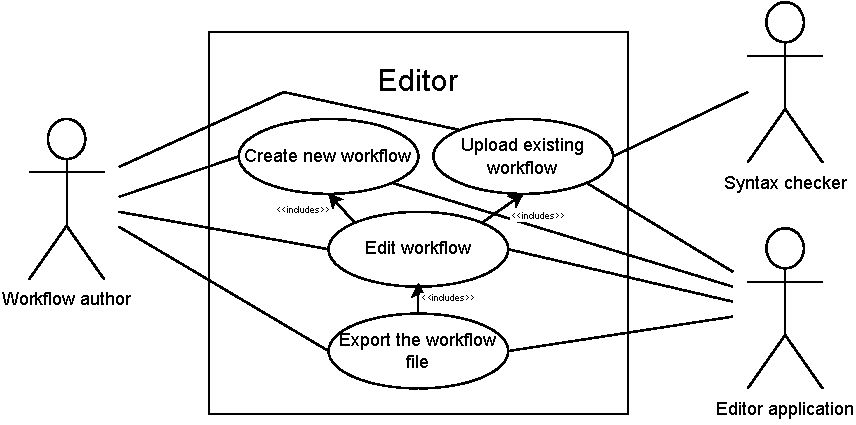
\includegraphics{./img/editorUC.pdf}
    \end{center}
    \caption{Editor - Use Case UML diagram}
\end{figure}
\end{center}

\clearpage
\subsection{Runner}

The \textit{Runner} is the part of the toolkit responsible for the automation execution.
The following section contains sample use cases, describing the standard user flow and exception handling.
If not stated otherwise, the user in the following examples corresponds to the \textit{User} user role. \

\setcounter{usecases}{1}

\def \usecase {Use Case \numb{usecases}}

\subsubsection*{\usecase: Running an automation}
\begin{itemize}
    \item \textbf{Goal}: User wants to run an automation.
    \item \textbf{Scenario}: 
    \begin{enumerate}[label=\arabic*.]
        \item User accesses the \textit{Runner} application.
        \item Using the \textit{Runner} interface, the user passes the automation to the \textit{Runner}.
        \item The \textit{Runner} validates the passed automation.
        \item The \textit{Runner} runs the automation, sharing the progress with the user.
        \item After the automation is done, the \textit{Runner} notifies the user, eventually presenting the results of the automation run.
    \end{enumerate}
    \item \textbf{Exception}: The file provided by the user in step 2 is not a valid automation file.
    \begin{itemize}
        \item \textbf{Exception flow}: The \textit{Runner} rejects such file with a detailed error message. 
        The \textit{Runner} interface returns to the initial state. The user can pass another automation file.
    \end{itemize}
\end{itemize}

\subsubsection*{\usecase: Stopping the execution early}
\begin{itemize}
    \item \textbf{Goal}: After submitting the automation to the \textit{Runner}, the user wants to stop the automation execution prematurely.
    \item \textbf{Scenario}: 
    \begin{enumerate}[label=\arabic*.]
        \item User accesses the \textit{Runner} application.
        \item Using the \textit{Runner} interface, the user passes the automation to the \textit{Runner}.
        \item The \textit{Runner} validates the passed automation.
        \item The \textit{Runner} runs the automation, sharing the progress with the user.
        \item Using the \textit{Runner} interface, the user orders the \textit{Runner} to stop the execution.
        \item The \textit{Runner} responds to the user's halt request. It stops the automation execution and exits gracefully. 
        The \textit{Runner} presents the user with the run results.
    \end{enumerate}
    \item \textbf{Note}: The run results (e.g. the data scraped from the websites) can be incomplete because of the early termination.
    Despite this, the early termination must not affect the data integrity.
\end{itemize}

\subsubsection*{\usecase: Debugging an automation}
\begin{itemize}
    \item \textbf{Goal}: An advanced user (see the \hyperref[DevUserRole]{Developer} user role) needs to gather information on their automation run performance.
    \item \textbf{Scenario}: 
    \begin{enumerate}[label=\arabic*.]
        \item User accesses the \textit{Runner} application. 
        \item Using the \textit{Runner} interface, the user passes the automation to the \textit{Runner}. The user also
        switches the debugging mode on.
        \item The \textit{Runner} validates the passed automation.
        \item The \textit{Runner} runs the automation, sharing the progress with the user.
        The \textit{Runner} now also shares the internal debugging information with the user. 
        \item After the automation is done, the \textit{Runner} notifies the user, presenting the debugging 
        and performance data. Eventually, it also presents the results of the automation run.
    \end{enumerate}
\end{itemize}

% \subsubsection*{\usecase: Running an automation within an initialized browser}
% \begin{itemize}
%     \item \textbf{Goal}: An advanced user (see the \hyperref[DevUserRole]{Developer} user role) wants to run an automation from a non-default browser context, e.g. on a specific page, or logged in to a certain web service.
%     \item \textbf{Scenario}: 
%     \begin{enumerate}[label=\arabic*.]
%         \item User accesses the \textit{Runner} application. 
%         \item Using the \textit{Runner} interface, the user passes the automation to the \textit{Runner}. 
%         Alongside the automation, the user also passes the browser context to the \textit{Runner}.
%         \item The \textit{Runner} validates the passed automation.
%         \item The \textit{Runner} runs the automation in the passed browser context, sharing the progress with the user.
%         \item After the automation is done, the \textit{Runner} notifies the user, eventually presenting them with the results of the automation run.
%         The \textit{Runner} also returns the now modified browser context.
%     \end{enumerate}
% \end{itemize}

\begin{center}
\begin{figure}[h!]
    \begin{center}
        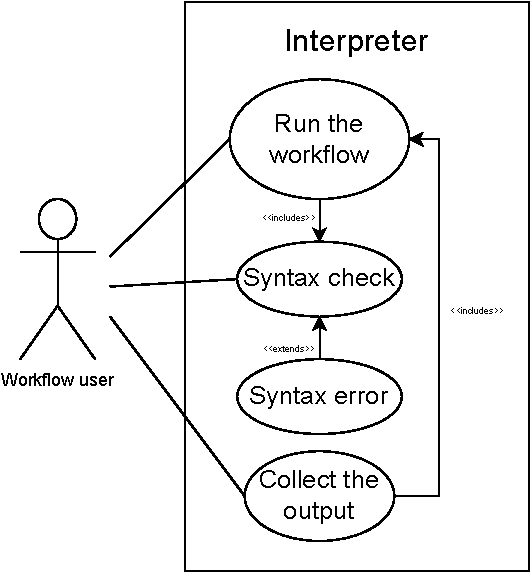
\includegraphics{./img/interpreterUC.pdf}
    \end{center}
    \caption{Interpreter - Use Case UML diagram}
\end{figure}
\end{center}